\begin{frame}{RDFS / OWL — the vocabulary model (L1)}
  \framesubtitle{Classes, properties, and how they relate}

  \begin{columns}[T]
    \begin{column}{0.56\textwidth}
      \centering
      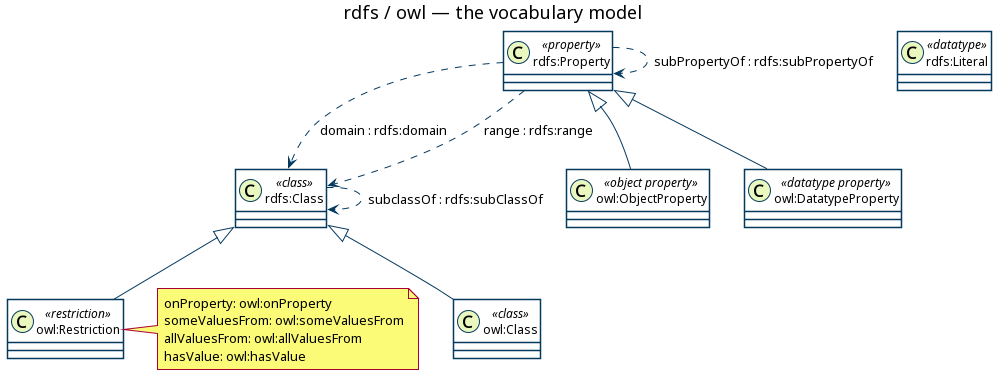
\includegraphics[width=\linewidth, height=0.6\textheight, keepaspectratio]{slides/im-101/rdfs-owl/figs/rdfs-owl.png}
    \end{column}
    \begin{column}{0.42\textwidth}
      \scriptsize
      \setlength{\itemsep}{0.5pt}
      \setlength{\parskip}{0pt}
      \textbf{Classes}
      \begin{itemize}
        \item \texttt{rdfs:Class}, \texttt{owl:Class} — \emph{sets} of resources
        \item \texttt{owl:Restriction} — anonymous classes
      \end{itemize}
      \vspace{0.4pt}
      \textbf{Properties}
      \begin{itemize}
        \item \texttt{owl:ObjectProperty} — links to a \emph{resource}
        \item \texttt{owl:DatatypeProperty} — links to a \emph{literal}
      \end{itemize}
      \vspace{0.4pt}
      \textbf{The glue}
      \begin{itemize}
        \item \texttt{rdfs:subClassOf} / \texttt{rdfs:subPropertyOf}
        \item \texttt{rdfs:domain} / \texttt{rdfs:range}
      \end{itemize}
      \vspace{2pt}
      \begin{alertblock}{}
        Open world: nothing is \emph{forbidden} unless you say so.
      \end{alertblock}
    \end{column}
  \end{columns}
\end{frame}
